\chapter{Conclusioni e sviluppi futuri}
Nel lavoro appena presentato è stata analizzata la rete ottenuta dall'analisi di 30 giorni di un server di Travian. I dati forniti possono essere rappresentati come un multi-grafo multi-layer per ognuno dei giorni considerati. Questi dati sono stati analizzati affrontando il problema secondo due approcci: aggregando i dati dei 30 giorni o mantenendo distinti i differenti giorni.
Per quanto concerne i dati aggregati, abbiamo valutato coefficienti di \textit{clustering} e centralità: i primi ci hanno permesso di concludere che il meccanismo di messaggistica diretta porti i nodi a contattare non solo i membri della sua alleanza, ma anche giocatori sconosciuti e non facenti parte della sua comunità. Allo stesso modo, per quanto riguarda gli scambi, troviamo un comportamento che mostra una forma di mercato “globalizzato”, senza un preferenza di interscambio con nodi conosciuti.
Per quanto riguarda le misure di centralità, betweenness e PageRank non hanno evidenziato nodi nettamente più rilevanti di altri. Ciò è ragionevole, in quanto, come già affermato, il meccanismo di messaggistica non richiede la presenza di tramiti o snodi, ma è possibile contattare direttamente ogni giocatore. Per quanto riguarda il layer dei \textit{trade}, emerge l'assenza della figura di “commerciante”; i nodi effettuano scambi direttamente, senza meccanismi preferenziali, semplicemente cercando il migliore affare disponibile.\\
L'analisi dell'andamento delle attività sul server durante i 30 giorni ha mostrato un progressivo calo del numero di giocatori, con un crollo sospetto avvenuto il 5 Dicembre. Non avendo informazioni aggiuntive circa possibili eventi esterni, non affermare con certezza quali siano le cause di questo evento, mentre l'andamento decrescente dell'attività è fisiologico in tutti i giochi di questo tipo.
Anche il numero di alleanze presenti sul server decresce costantemente, ma il rapporto tra le alleanze con un numero di membri significativo e il numero di alleanze totali rimane pressoché stabile.\\
La ricerca di comportamenti sospetti dei giocatori non ha evidenziato la presenza di \textit{spammer} sul server, avallando la tesi dell'implementazione di un ottimo filtro integrato nel sistema di messaggistica. Al contrario, sono stati individuati alcuni giocatori con comportamenti sospetti per quanto riguarda l'utilizzo di \textit{side-village}, l'approfondimento di tale comportamento richiederebbe un'analisi più estesa e la consultazione con degli esperti di dominio, oltre a un eventuale intervento da parte degli amministratori del server per la punizione di tali giocatori.\\
Ci siamo infine concentrati sullo studio dei meccanismi interni alle community, analizzando densità e reciprocità medie. Questo ci ha permesso di rilevare una tendenza all'intensa interconnessione nel layer delle comunicazioni, mentre per quanto concerne i \textit{trade}, vi è una forte presenza di donazioni tra membri, mentre i commerci non sono così frequenti.
Approfondendo l'analisi sull'alleanza principale, abbaino ripetuto le misure di centralità sui membri, individuando alcuni nodi con valori sensibilmente maggiori di altri. Essi, identificati come i vertici della comunità, sono numericamente molto inferiori rispetto al totale, ma trovano associati valori di centralità più elevati. Si delinea quindi una struttura di gestione piramidale dell'alleanza. Troviamo differenze anche per quanto riguarda la densità di messaggi e \textit{trade}, delineando l'immagine di una community più connessi della media.\\
Abbiamo infine analizzato i meccanismi di interazione presenti tra le 4 più grandi alleanze sui vari layer. Per quanto riguarda gli attacchi, la tendenza emersa è quella di non aggressione, preferendo concentrare gli attacchi su obiettivi più facile e ricchi di bottino. Anche lo scambio di messaggi si è rivelato essere molto fitto all'interno della comunità e poco all'esterno, con la presenza di un numero molto ristretto di nodi diverse comunità che comunicano tra loro (possibili ambasciatori o spie). Per quanto riguarda gli scambi, è stata confermata l'dea di un mercato unico data la presenza di una rete di scambi tra i membri delle varie comunità. Un'aspetto interessante emerso dalla rappresentazione del layer delle comunicazioni è la presenza di due alleanze fortemente connesse, quasi a formare una comunità unica. L'ipotesi avanzata è che si possa trattare di una macro alleanza o di un meccanismo accademia-principale.

Di seguito proponiamo alcuni possibili sviluppi futuri durante lo svolgimento di questo lavoro:
\begin{itemize}
	\item individuazione di figure all'interno di un'alleanza quali: spie, reclutatori, ambasciatori, \textit{leader}\dots;
	\item identificare il comportamento dei nodi appartenenti a un'alleanza che si disgrega: “cercano una nuova community, rimangono nodi isolati oppure avevano già preso contatti con altre alleanza?”. Un'analisi più approfondita delle misure di centralità potrebbe suggerire le figure sospette;
	\item ricerca di sotto-strutture all'interno delle varie alleanze;
	\item sviluppo di un meccanismo per l'individuazione di gerarchie accademia-principale;
	\item effettuare attività di predizione sull'evoluzione delle alleanze e delle relative interazioni.
\end{itemize}

\begin{appendices}
\section*{Appendice A}
\label{append}
In questo appendice sono riportate alcune immagine extra ottenute durante il nostro lavoro di analisi ma che non ci sono sembrate sufficientemente rilevanti da essere inserite nella relazione.
\begin{figure}[b!]
	\centering
	\subfloat[Distribuzone degli \textit{outlier} nel grafo aggregato dei 30 giorni per la misura \textit{out-degree} nel layer degli attacchi.]{%
		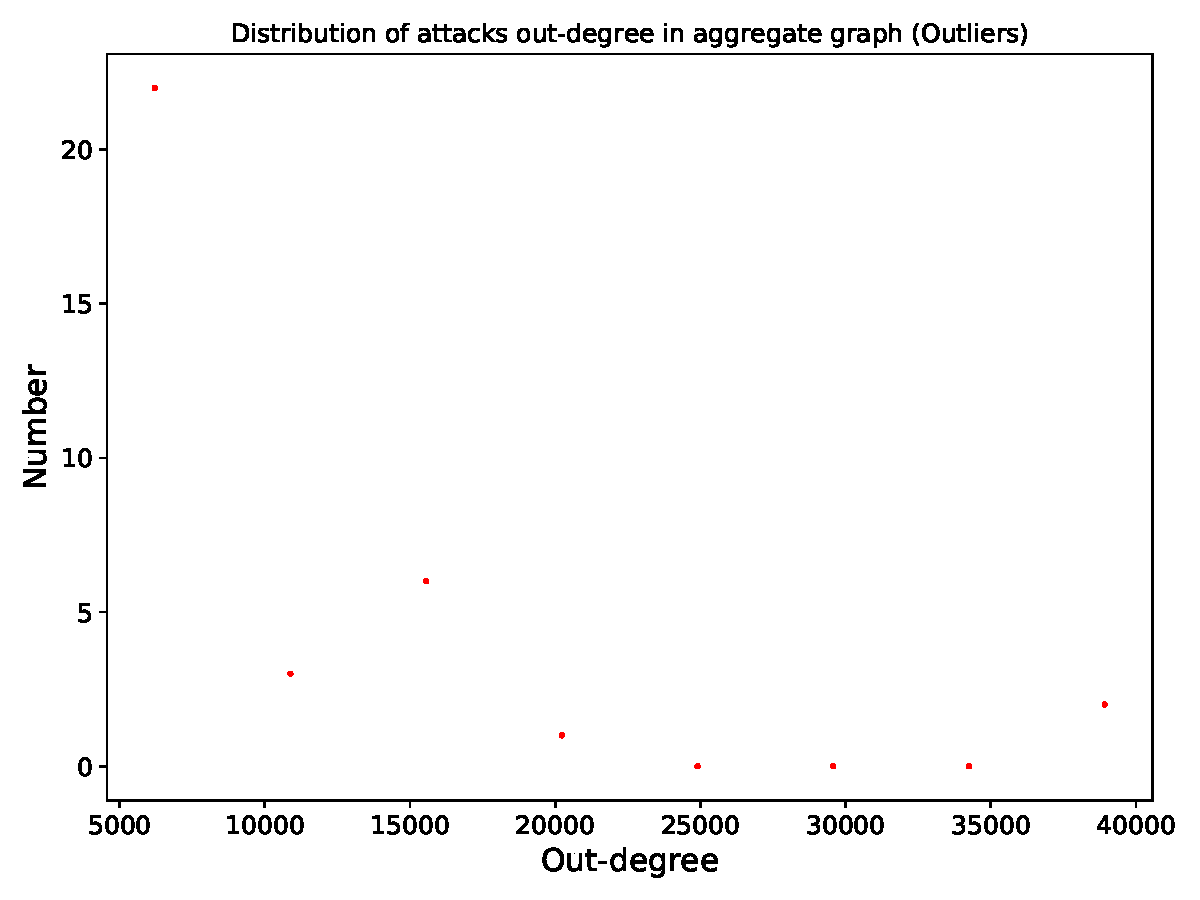
\includegraphics[width=.55\linewidth]{images/Outliers/attacks_out_degree_outliers}
	}%
	\subfloat[Distribuzone degli \textit{outlier} nel grafo aggregato dei 30 giorni per la misura di grado complessivo nel layer degli attacchi.]{%
		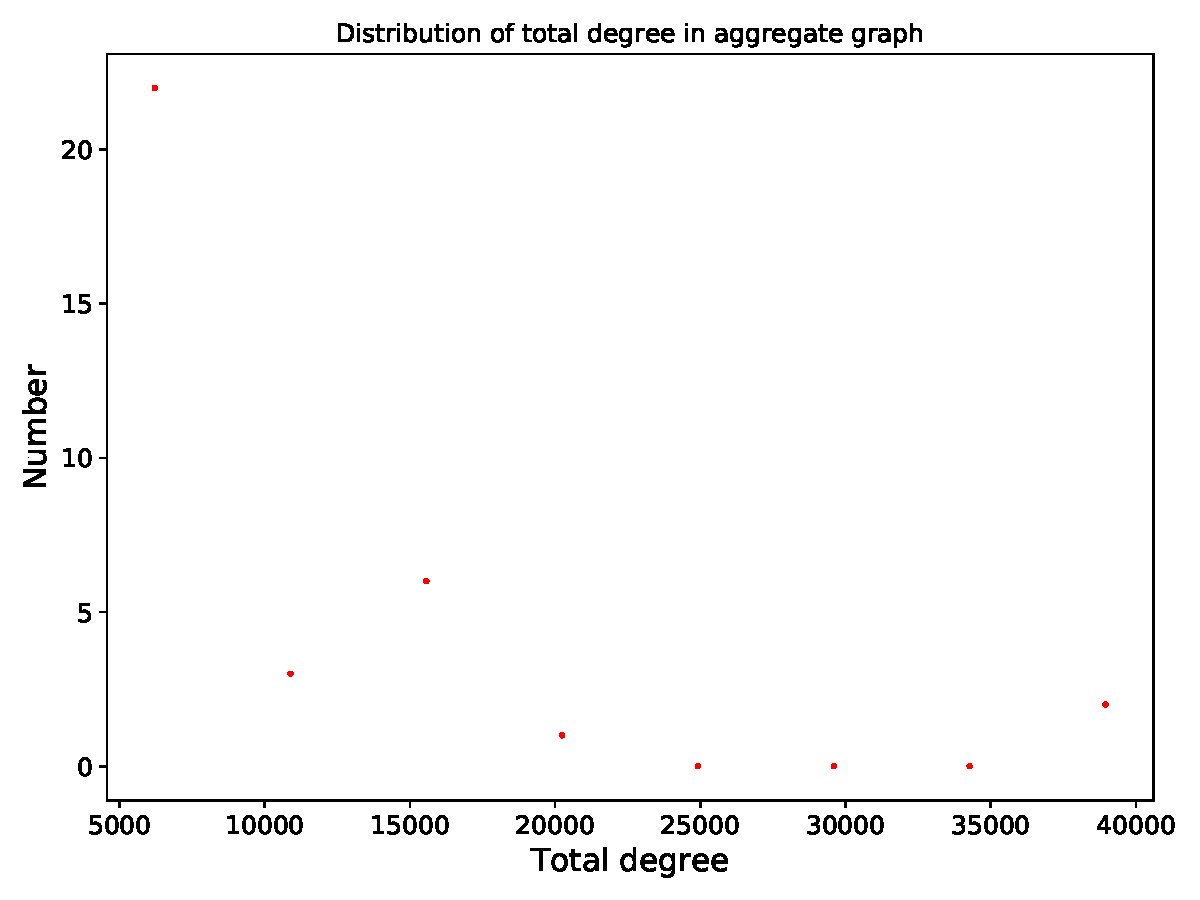
\includegraphics[width=.55\linewidth]{images/Outliers/attacks_total_degree_outliers}
	}\\
	\subfloat[Distribuzone degli \textit{outlier} nel grafo aggregato dei 30 giorni per la misura \textit{out-degree} nel layer dei messaggi.]{%
		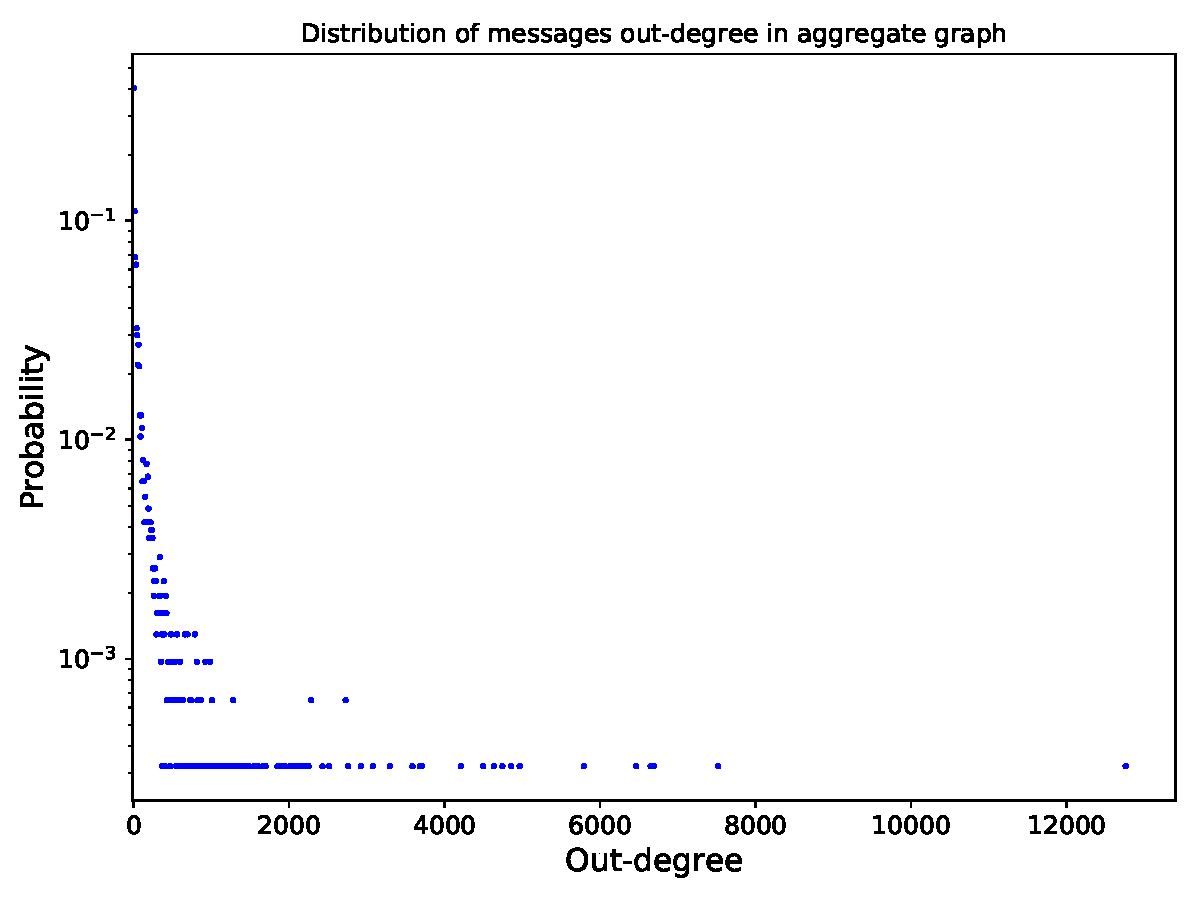
\includegraphics[width=.55\linewidth]{images/Outliers/messages_out_degree_outliers}
	}%
	\caption{Distribuzioni degli \textit{outlier} per alcuni layer del grafo aggregato sui 30 giorni.}
\end{figure}

\begin{figure}
	\subfloat[Distribuzione dell'\textit{in-degree} medio sui 30 giorni dei nodi dell'alleanza principale.]{%
		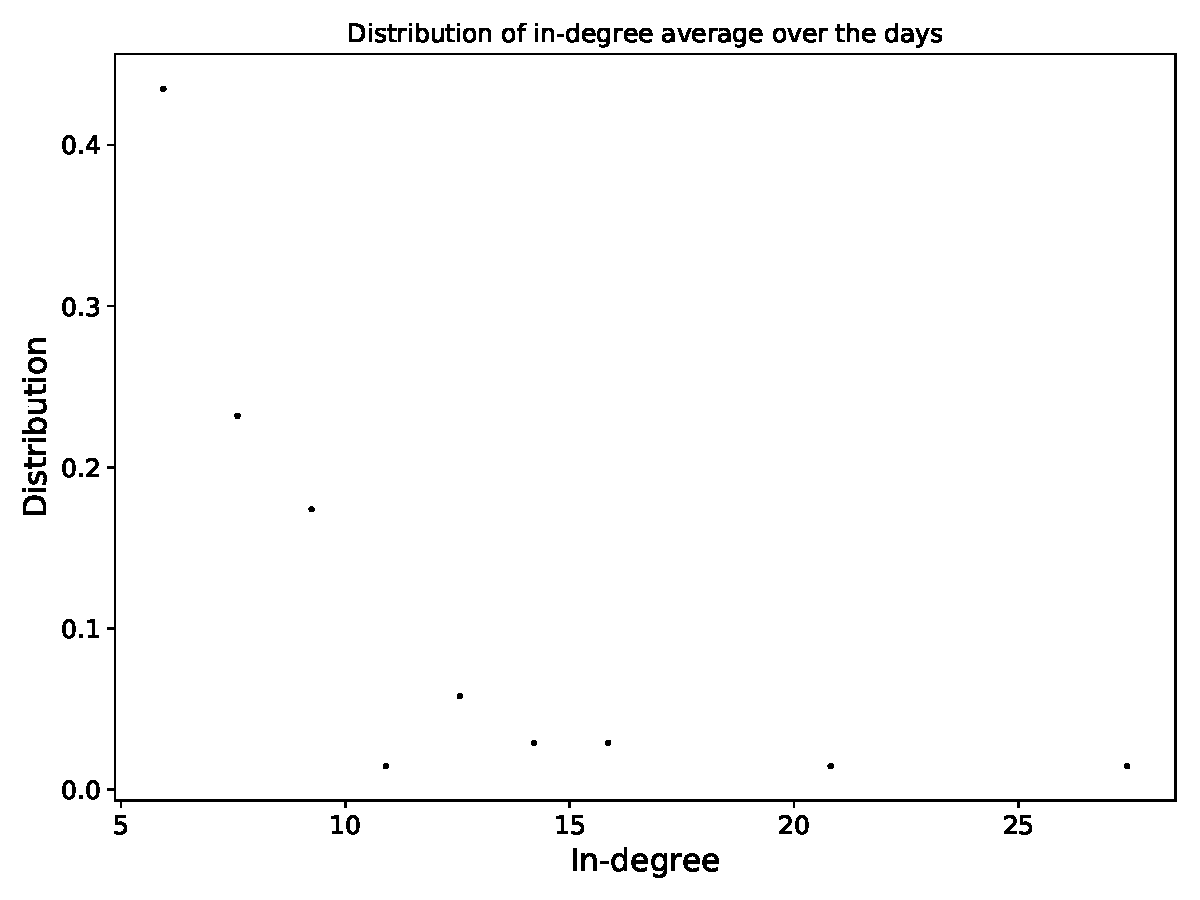
\includegraphics[width=.48\linewidth]{images/Outliers/in-degree_distribution_mrc_mean}
	}
	\hfill
	\subfloat[Distribuzione di \textit{in-degree} di ogni nodo sui 30 giorni dei nodi dell'alleanza principale.]{%
		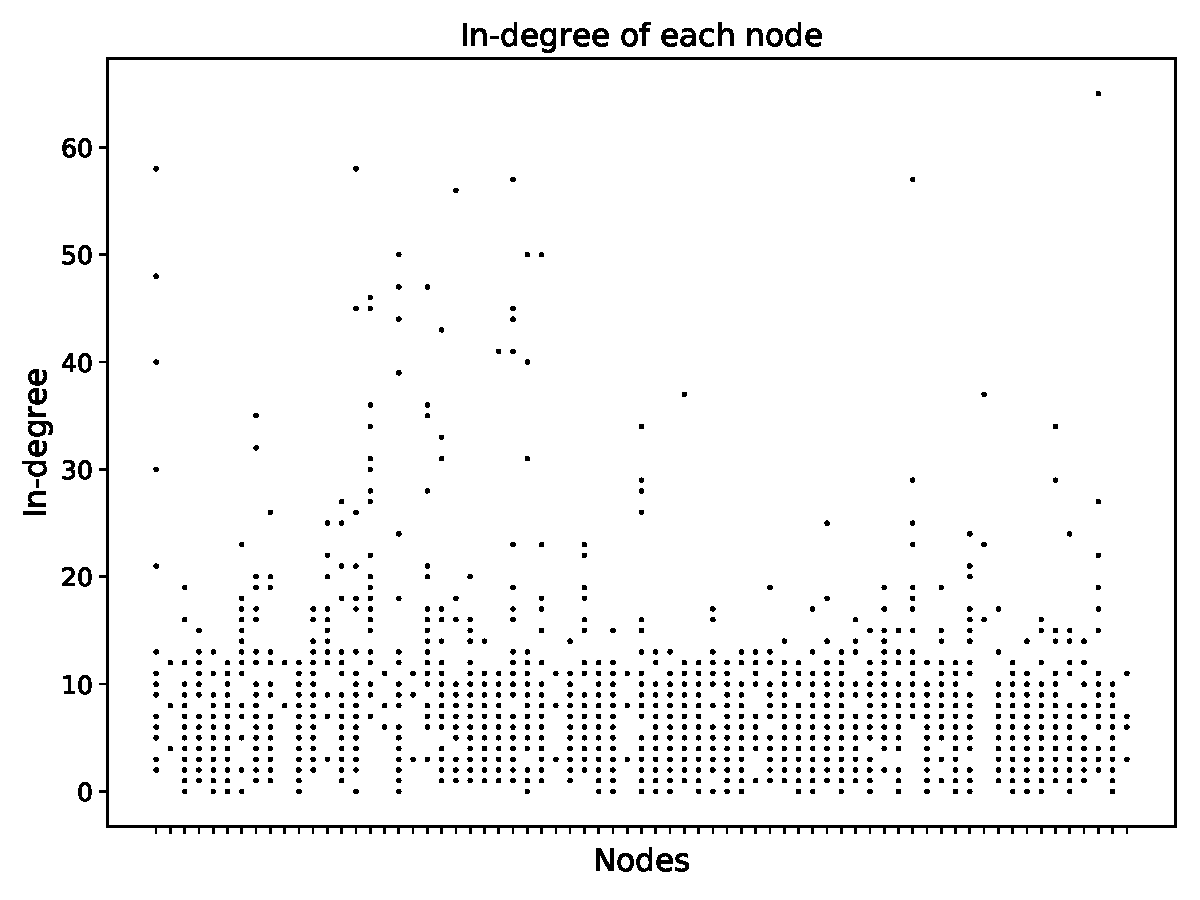
\includegraphics[width=.48\linewidth]{images/Outliers/in-degree_distribution_mrc_30}
	}
	\caption{Analisi dell'\textit{in-degree} medio e di ogni nodo sui 30 giorni per i nodi dell'alleanza principale.}
\end{figure}


\end{appendices}
